\chapter*{Введение}                         % Заголовок
\addcontentsline{toc}{chapter}{Введение}    % Добавляем его в оглавление
\newcommand{\me}{m_\mathrm{e}}
\newcommand{\wpl}{\omega_\mathrm{p}}
Как известно~\cite{Mikhailovsky1971}, в условиях анизотропного распределения частиц по скоростям плазма является неравновесной и в ней может развиваться ряд кинетических неустойчивостей, приводящих к возникновению хаотических электромагнитных полей и согласованной с ними плазменной турбулентности. Такая ситуация характерна для широкого круга задач физики бесстолкновительной плазмы, космической и лазерной, в которой время свободного пробега частиц много больше времени развития подобной турбулентности~\cite{Baumjohann2012, Treumann2009, Marcowith2016}. Настоящая работа посвящена анализу квазимагнитостатической турбулентности, обусловленной апериодической неустойчивостью вейбелевского типа~\cite{Weibel1959, Fried1959, Kocharovsky2016}, которая обладает одним из наибольших инкрементов среди различных неустойчивостей неравновесной анизотропной плазмы. 

Неустойчивость, впервые предсказанная Вейбелем в 1959 году~\cite{Weibel1959}, имеет простую физическую интерпретацию, предложенную Фридом~\cite{Fried1959}. В своей работе он рассмотрел суперпозицию двух противоположно направленных потоков холодной плазмы в присутствии слабого, периодического в пространстве магнитного поля (одной из гармоник шумов, присущих реальной плазме): электроны из встречных потоков смещались под действием силы Лоренца в разные стороны, что приводило к образованию токовых филаментов, которые в свою очередь способствовали экспоненциальному росту магнитного поля. 

В линейном приближении вейбелевская неустойчивость как в кинетическом подходе к описанию бесстолкновительной плазмы, так и в гидродинамическом приближении весьма подробно изучена; см., например,~\cite{Kocharovsky2016}. Изучение нелинейной стадии проводилось в ряде работ, в том числе в гидродинамическом приближении, прежде всего, в случае двухпучкового распределения частиц (например,~\cite{Romanov2004,Bychenkov2003}). Однако в более адекватном кинетическом подходе данная задача остается мало изученной. В настоящей работе с целью исследования процессов, происходящих на нелинейной стадии неустойчивости, проведено численное исследование эволюции связанных пространственных гармоник возмущений функции распределения (ФР) частиц и магнитного поля в анизотропной бесстолкновительной плазме в рамках двумерной постановки задачи с различными начальными анизотропными распределениями частиц по скоростям (рис. \ref{fig:GeomIsolines}). ТМ-вейбелевская неустойчивость насыщается, т.\,е. прекращается рост среднеквадратичного магнитного поля, тогда, когда оно в достаточной мере выравнивает средние значения продольной ($T_{\|}$, вдоль оси $y$) и поперечной ($T_\perp $, вдоль оси $x$ или в плоскости $x,z$ в зависимости от постановки задачи) эффективных температур, так что его присутствие, пространственная неоднородность и особенно понизившийся и тоже неоднородный уровень анизотропии $A={T_{\|}}/{T_{\perp}}-1$ исключают экспоненциальное нарастание каких-либо возмущений, в том числе крупномасштабных (см.,~например,~\cite{Borodachev2016_Radiofiz}). В дальнейшем уровень турбулентности медленно понижается и её пространственный спектр постепенно эволюционирует в длинноволновую область спектра.

Слабо столкновительная плазма с анизотропным распределением частиц по скоростям является неравновесной~\cite{Mikhailovsky1971,Krall1973}, и развивающиеся кинетические неустойчивости формируют в ней хаотические электромагнитные поля и согласованную с ними плазменную турбулентность. Ее динамика и свойства определяются нелинейными эффектами, которые во многих случаях хотя и являются не сильно выраженными, но для полноценного описания требуют трудоемких расчетов кинетики огромного числа частиц (при этом моделирование наиболее эффективным методом частиц в ячейках~\cite{Kato2005,Borodachev2010,Ruyer2015,Lazar2022,Borodachev2016_Radiofiz,Romanov2004} вносит численный шум, неизбежно искажающий результаты). Такая ситуация характерна для широкого круга задач физики разреженной космической, лазерной и газоразрядной плазмы, в которой время свободного пробега частиц много больше времени развития подобной слабо нелинейной турбулентности~\cite{Baumjohann2012,Treumann2009,Marcowith2016,Gary1993}. 

Среди неустойчивостей анизотропной плазмы апериодическая неустойчивость вейбелевского типа~\cite{Weibel1959,Zhou2022,Fried1959,Kalman1968,Morse1971,Kocharovsky2016,Lazar2006,Stockem2009,SchaeferRolffs2006} обладает одним из наибольших инкрементов и вместе с тем не сопровождается сильными резонансными нелинейными эффектами, поскольку ограничивается формированием квазимагнитостатических филаментов тока и не приводит к непосредственному возбуждению каких-либо волн. Настоящее исследование посвящено нелинейной стадии ее развития и описанию эволюции спектра возникающей турбулентности в простейших постановках 1- и 2-мерных задач на основе разработанного авторами численного кода, реализующего квазилинейный подход к расчету динамики вейбелевских мод~\cite{Kuznetsov2022}. Он учитывает основные нелинейные явления в указанной задаче и позволяет сразу находить представляющий физический интерес спектр полей и токов, избегая моделирования кинетики частиц. Анализ этого спектра актуален для физики звездного ветра, ударных волн в космической плазме, токовых структур, возникающих при лазерной абляции, и др.; см., например,~\cite{Lazar2022,Romanov2004,Medvedev2005,Chatterjee2017}.

В линейном приближении вейбелевская неустойчивость изучена достаточно подробно, особенно для бимаксвелловского распределения частиц~\cite{Weibel1959,Fried1959,Vagin2014}. Существующая полностью аналитическая квазилинейная теория эволюции вейбелевской турбулентности разработана лишь в одномерной (1D2V) геометрии, причем для весьма ограниченной области параметров и без должного описания временной эволюции~\cite{Pokhotelov2011}. Полуаналитическое решение системы квазилинейных уравнений в 1D3V геометрии~\cite{Ruyer2015} с опорой на эмпирические данные численного моделирования также применимо лишь для небольшой области параметров плазмы. 

В развиваемом численном квазилинейном подходе функция распределения частиц и электрическое и магнитное поля представлены в виде сумм пространственных мод (гармоник), удовлетворяющих самосогласованным квазилинейным уравнениям, в которых все нелинейные явления обусловлены совместным действием мод на форму средней по пространству функции распределения частиц по скоростям. Последняя определяет текущие значения инкрементов (декрементов) и, возможно, действительных частот всех рассматриваемых мод, в остальном эволюционирующих независимо. В результате, в отличие от метода частиц в ячейках, кардинально снижается уровень шумов и удается получать спектры вейбелевской турбулентности в гораздо более высоком качестве и в недоступных ранее областях параметров, правда, ценой потери некоторых слабых нелинейных эффектов при использовании сравнимых или даже б\'{о}льших вычислительных ресурсов.

Для определенности в конкретных расчетах ниже будем выбирать начальную функцию распределения частиц по скоростям бимаксвелловской, считая температуру частиц наибольшей вдоль оси $y$, называемой осью анизотропии. Для простоты будем предполагать плазму и все поля в ней однородными вдоль этой оси, т.е. решать систему уравнений Максвелла~-- Власова~\cite{Baumjohann2012} в одном (по координате $x$) или двух (по координатам $x$ и $z$) измерениях, а следовательно, полагать нулевой проекцию волновых векторов мод $\vec{k}$ на ось анизотропии: $k_y=0$. При этом в каждой моде электрическое поле $\vec{E}$ направлено вдоль оси анизотропии, а магнитное $\vec{B}$ ортогонально ей и волновому вектору $\vec{k}$ (ТЕМ-моды). 

Главная цель представленной работы состоит в изучении нелинейных явлений квазилинейного типа, доминирующих в процессе развития вейбелевской турбулентности. Насколько нам известно, последовательный квазилинейный анализ ее эволюции до сих пор никем не проводился ни для какой анизотропии начальной функции распределения частиц по скоростям (ср., например,~\cite{Ruyer2015,Pokhotelov2011,Davidson1972}). Более того, другими авторами не проводилось даже достаточно длительное моделирование динамики спектра вейбелевских мод в простейшей постановке задачи об одномерной (1D2V) и аксиально симметричной двумерной (2D3V) турбулентности, рассматриваемых в настоящей работе. Вместе с тем, некоторые выявленные нами особенности эволюции спектра и динамики отдельных мод аналогичны численно найденным ранее в других постановках задачи о вейбелевской турбулентности.

Следует отметить, что полноценное (3D3V) долговременное компьютерное моделирование изучаемых турбулентных явлений пока невозможно из-за недостаточной мощности вычислительных ресурсов. В ограниченных расчетах методом частиц в ячейках, проведенных в данной работе и ранее, далеко не всегда удается выделить слабые нелинейные эффекты, например, четырехволновое взаимодействие мод, на фоне более сильных квазилинейных эффектов и трудно отделимых неизбежных компьютерных шумов. Подобное выделение стало возможным только недавно и осуществлено в единичных случаях при специальных условиях для нестандартных задач (см.~\cite{Garasev2018,Garasev2021}), так что ниже оно затрагивается лишь вскользь.

Развитие магнитной турбулентности в помещенной во внешнее однородное магнитное поле $\vec{B}_{ext}=(0, 0, B_{ext})$ бесстолкновительной плазме на временах, допускающих пренебрежение движением тяжелых ионов, описывается известными уравнениями  Максвелла--Власова~\cite{???}. Они имеют следующий вид  для электрического $\vec{E}(\vec{r}, t)$ и магнитного $\vec{B}(\vec{r}, t)$ полей и функции распределения электронов $f(\vec{v},\vec{r}, t)$, зависящих от времени $t$, радиуса-вектора $\vec{r}=\left(x,y,z\right)$ и скорости $\vec{v}=\left(v_x,v_y,v_z\right)$
\begin{align}
     \label{eq:maxw1} 
    \nabla \times \vec{B}=\dfrac{1}{c}\dfrac{\partial \vec{E}}{\partial t}+\dfrac{4\pi}{c}\vec{j}, \\
    %
    \label{eq:maxw2}
    \nabla \times \vec{E}=-\dfrac{1}{c}\dfrac{\partial \vec{B}}{\partial t}, \\
    %
    \dfrac{\partial f}{\partial t}+\vec{v}\dfrac{\partial f}{\partial \vec{r}}-\dfrac{e}{\me} \left(\vec{E}+\dfrac{1}{c}\left[\vec{v},\vec{B}+\vec{B}_{ext}\right]\right) \dfrac{\partial f}{\partial \vec{v}}=0,
    \label{eq:Vlasov}
\end{align}
где $c$~-- скорость света в вакууме, $e$ и $\me$~-- величина заряда и масса электрона, $\vec{j}=-e\iiint^{+\infty}_{-\infty}\vec{v}f(\vec{v},\vec{r}, t) d^3\vec{v}$~-- плотность тока, $N=\iiint^{+\infty}_{-\infty}f(\vec{v},\vec{r}, t) d^3\vec{v}$~-- концентрация электронов, $N_0$~-- ее начальное однородное значение. Для определенности полагается, что в начальный момент времени нормированная функция распределения электронов по скоростям $\Psi = c^3f/N_0$ имеет бимаксвелловскую форму, вытянутую вдоль оси $z$, т.е. вдоль внешнего магнитного поля:


\begin{equation}
\label{bimax}
\Psi(\vec{\beta})=\dfrac{1}{\pi^{3/2}\beta_{\perp 0}^2 \beta_{\| 0} } \exp\left(-\dfrac{\beta_x^2+\beta_y^2}{\beta_{\perp 0}^2}-\dfrac{\beta_z^2}{\beta_{\| 0}^2}\right).
\end{equation}

Здесь $\beta_{x,y,z}={v_{x,y,z}}/{c}$, т.\,е. $\vec{\beta}=\vec{v}/{c}$. Ниже используется начальное значение параметра анизотропии $A_0={\beta^2_{\| 0}}/{\beta^2_{\perp 0}}-1 > 0$, определяемое различием исходных тепловых скоростей вдоль и поперек внешнего магнитного поля. Рассматриваемая задача, хотя и является трехмерной, обладает аксиальной симметрией. Поскольку полноценные трехмерные расчеты требуют больших вычислительных затрат, целесообразно выяснить, какие параметры турбулентности и на каких временах могут быть определены из двумерных расчетов. С этой целью в работе проведено сравнение результатов расчетов в трехмерной (3D3V) и двух вариантах двумерной (2D3V) геометриях. Во всех случаях проводится динамический учет всех трех компонент скорости частиц $\vec{v}$ и зависящих от них полей.  Ограничением в двумерных расчетах являются лишь исключенные зависимости исследуемых функций либо от координаты $y$  в $(x,z)$ -- геометрии, когда магнитное поле и ось анизотропии лежат в плоскости расчета $xz$, либо от координаты $z$ в аксиальной $z$-геометрии, когда магнитное поле и ось анизотропии ортогональны плоскости расчета $xy$.  В отличие от второго варианта, когда отсутствуют наклонные к магнитному полю моды и имеется аксиальная симметрия задачи, в первом.... усложняет динамику турбулентности, описание которой в 2D3V ..... становится некорректным в сравнении с полноценным трехмерным расчетом.
 
В работе используются обезразмеренные значения времени, волнового числа и амплитуд мод магнитного поля~(\ref{eq19plus1}):
\begin{equation}
\label{eq19plus1}
   \tau=\wpl t, \
    K=\dfrac{kc}{\wpl}, \  b_{K_{n}}=\dfrac{B_{K_{n}}}{\sqrt{8\pi N T_{\|0}}},\ 
    \wpl^2=\dfrac{4\pi Ne^2}{\me},\
    T_{\|0}=\dfrac{m_ec^2\beta_{\|0}^2}{2},
\end{equation}
Температура измеряется в энергетических единицах, т.е. с учетом постоянной Больцмана $k_B$. Для описания эволюции однородной компоненты распределения частиц по скоростям $f_0(t,\overrightarrow{\beta})=\iiint\limits^{\infty}_{-\infty}f(\vec{v},\vec{r}, t) d^3\vec{r}$ вводится относительная поправка к ней и эффективный параметр анизотропии:
\begin{equation}
\label{eq19plus2}
    \delta f_{0}(t,\overrightarrow{\beta})=\frac{f_0(t,\overrightarrow{\beta})-f_0(0,\overrightarrow{\beta})}{f_0(0,0)},\ A=\frac{2\iiint\limits^{\infty}_{-\infty}\beta_z^2f_{0}(\tau,\overrightarrow{\beta}) d\beta_x d\beta_yd\beta_z}{\iiint\limits^{\infty}_{-\infty}\left(\beta_x^2+\beta_y^2\right)f_{0}(\tau,\overrightarrow{\beta}) d\beta_x d\beta_y d\beta_z}-1 .   
\end{equation}
Кроме выявления динамики указанных величин~(\ref{eq19plus2}), представленные ниже расчеты призваны выявить закономерности в эволюции турбулентных магнитных и электрических полей и плотности тока электронов, а также пространственных спектров данной турбулентности.

Ключевыми параметрами в рассматриваемой начальной задаче о магнитной турбулентности являются начальная анизотропия $A_0$ распределения электронов по скоростям и нормированное внешнее магнитное поле $b_{ext}=B_{ext}/\sqrt{8\pi N T_{\|0}}\lesssim1$, равное обратному квадратному корню из плазменного бета-параметра. Данные величины не только задают диапазон первоначально неустойчивых мод, но и определяют дальнейшую нелинейную эволюцию спектра. В отсутствие магнитного поля имеется  апериодическое нарастание лишь ТМ-мод,  магнитное поле которых ортогонально плоскости, определяемой волновым вектором и осью анизотропии. При заданной величине поперечной компоненты волнового вектора наибольшими инкрементами обладают поперечные моды, волновые вектора которых перпендикулярны к оси анизотропии. Для них диапазон неустойчивости включает волновые числа в промежутке $\left(0;\sqrt{A_0}\right)$.\cite{??} При $A_0\ll1$ максимальный инкремент (в единицах $\omega_p$) равен $\gamma_\mathrm{max}\approx 2 \beta_{\perp0} (A_0 / 3)^{3/2}$ и достигается для оптимального волнового числа $K_\mathrm{\perp opt} \approx (A_0 / 3)^{1/2}$. При $A_0 \gg 1$ имеем $\gamma_\mathrm{max} \approx \beta_{\perp0} \left( \left[ (A_0+1)/2 \right]^{1/2} - 1 \right)$ для оптимального волнового числа $K_\mathrm{\perp opt} \approx \left( \left[ (A_0+1)/2 \right]^{1/2} - 1 \right)^{1/2}$~(рис. \ref{ris:mode_coupling}a).
\begin{figure}[h]

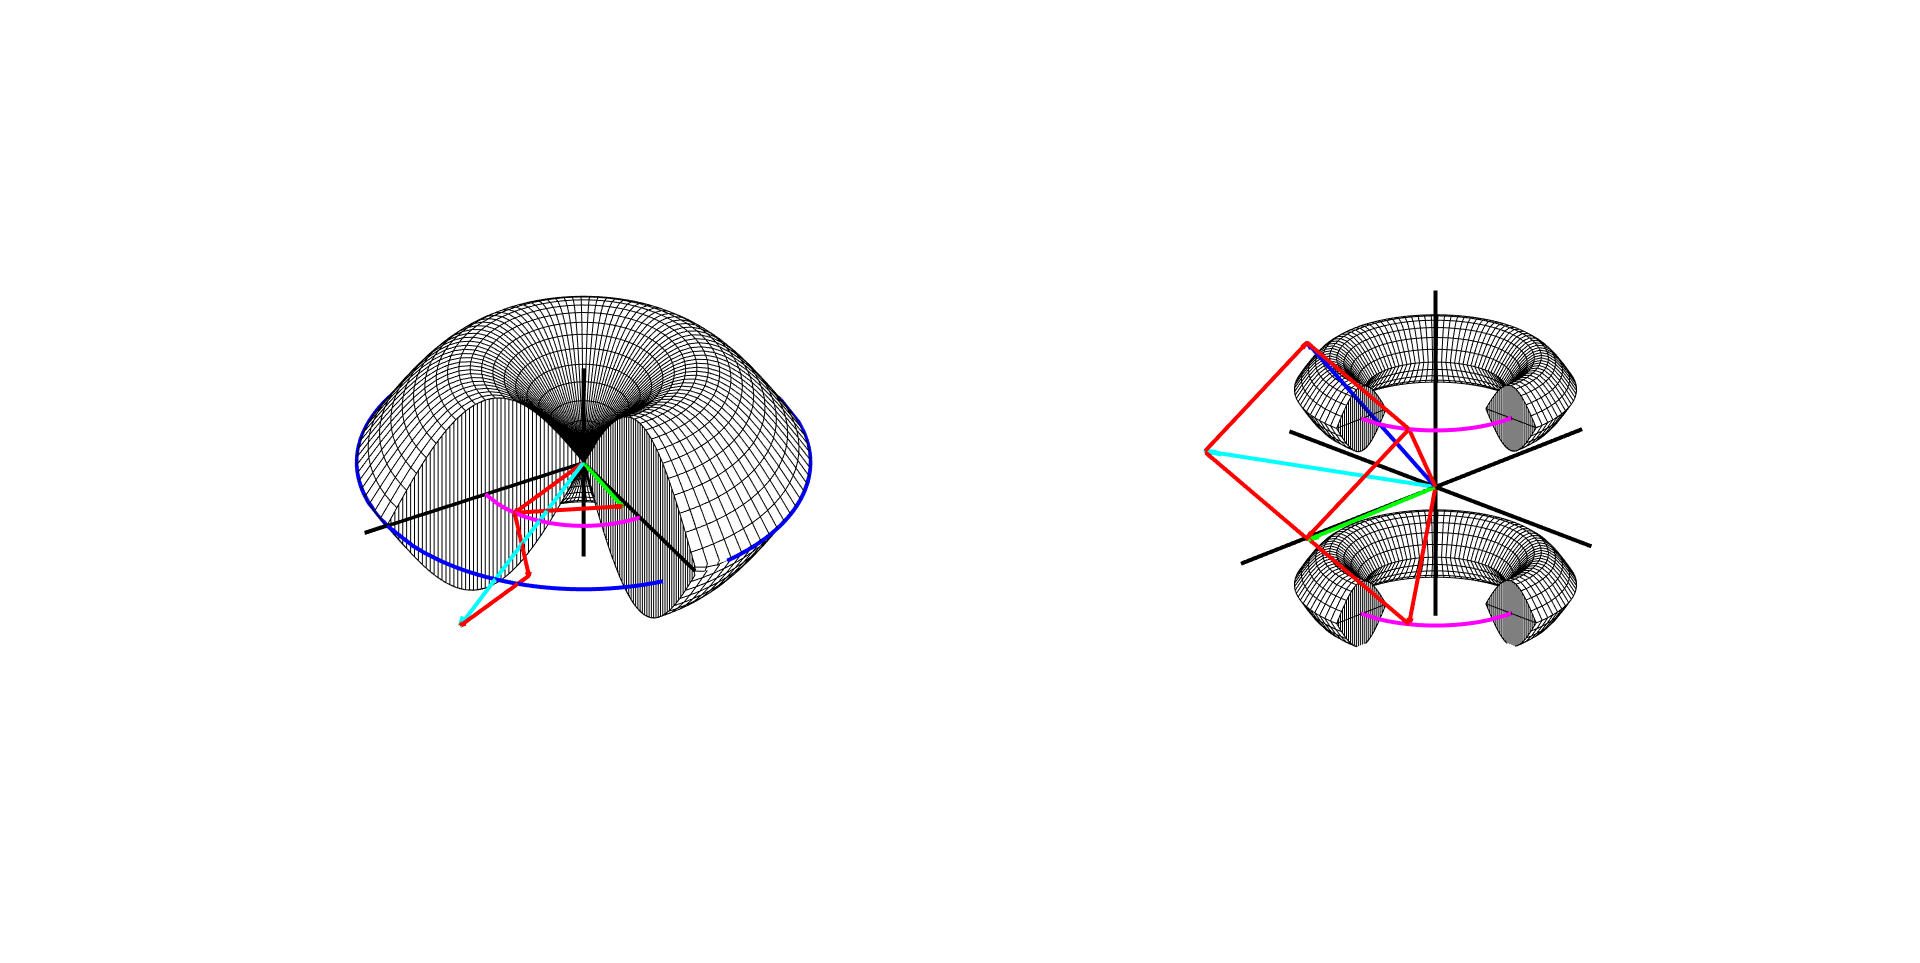
\includegraphics[width=1\linewidth]{introduction/mode_coupling.png}
\captionstyle{normal}
\caption{Трехмерная иллюстрация области апериодической неустойчивости в пространстве волновых векторов (a) в отсутствие внешнего магнитного поля и (b) в достаточно сильном внешнем магнитном поле. Синяя линия соотвествует границе неустойчивости поперечных мод $|K_\perp|=\sqrt{A}$ в отсутствие внешнего магнитного поля, а розовая линия~-- оптимальным модам $\overrightarrow{K}_{opt}$. Красные линии демонстрируют примеры оптимальных волновых векторов, взаимодействие которых в значительной степени определяет генерацию мод (зеленый, бирюзовый и синий цвет) вне области линейной неустойчивости.
}
\label{ris:mode_coupling}
\end{figure}

В присутствии внешнего магнитного поля $b_{ext}$ имеются две неустойчивые ветви: так называемые "периодическая"~ и "апериодическая"\cite{???}. Моды, направленные преимущественно вдоль внешнего магнитного поля, а значит, и оси анизотропии, относят к периодическим, поскольку их линейный инкремент мал в сравнении с действительной частотой и в сравнении с линейным инкрементом мод другой ветви~\cite{Li2000}. Поэтому влияние "периодической"~ ветви фактически не проявляется в расчетах методом частиц в ячейках, проводимых в настоящей работе, и не учитывается в приближенном квазилинейном описании.

Другую ветвь неустойчивости в литературе принято называть апериодической~\cite{???}, хотя нами показано, что в определенных условиях у ее линейно поляризованных мод присутствует действительная частота, увеличивающаяся с ростом внешнего магнитного поля $B_{ext}$ и уменьшением угла $\theta$ между волновым вектором $\vec{K}$ и этим магнитным полем. Область неустойчивости поперечных мод с увеличением внешнего поля достаточно быстро сужается,  как с длинноволновой, так и с коротковолновой стороны спектра, а линейный инкремент всех мод, остающихся неустойчивыми, уменьшается. В работе~\cite{Emelyanov2023_Radiophys} в пределе $\gamma\ll K_\perp\beta_\perp$, реализующемся при невысокой начальной анизотропии ($A_0\lesssim1$), либо при высокой анизотропии и внешнем магнитном поле, близком к подавляющему, область неустойчивости поперечных мод оценивалась как:
\begin{equation}
    K_\perp\in\left(\frac2{\sqrt{3}}\sqrt{A_0}\cos\left[\frac{\pi}3+\frac13\arccos\left(\frac{b_{ext}}{b_{s\perp}(A_0)}\right)\right];\frac2{\sqrt{3}}\sqrt{A_0}\cos\left[\frac{\pi}3-\frac13\arccos\left(\frac{b_{ext}}{b_{s\perp}(A_0)}\right)\right]\right),
    \label{eq:border_perp_inst}
\end{equation}
где $b_{s\perp}(A_0)$~--- нормированное магнитное поле, подавляющее неустойчивость поперечных мод, квадрат которого оценен в~\cite{Emelyanov2023_Radiophys} как:
\begin{equation}
    b_{s\perp}^2(A_0)=\frac{8\pi}{27}\frac{A_0^3}{1+A_0^3}<1.
    \label{eq:Emel_condition}
\end{equation}
По мере увеличения внешнего магнитного поля $b_{ext}$ монотонно уменьшается не только линейный инкремент всех поперечных мод, но и угол между внешним магнитным полем и волновым вектором моды с наибольшим инкрементом~(рис. \ref{ris:mode_coupling}b)~\cite{Moya2022,Li2000,Camporeale2008}. Таким образом, для наклонных мод неустойчивость может развиваться при $b_{ext}>b_{s\perp}(A_0)$. Вводя величину магнитного поля $b_s(A_0)$, при которой апериодическая неустойчивость полностью подавлена, приведем оценку для неё из работы~\cite{Hellinger2014}, аппроксимирующую численно полученный порог неустойчивости в диапазоне значений начальной анизотропии $A_0$ от $0.2$ до $9$:

\begin{equation}
    b_{s}^2(A_0)=\left(\frac{A_0}{1.27(1+A_0)}\right)^{\frac1{0.954}}.
    \label{eq:Hellinger_condition}
\end{equation}
\begin{figure}[h]

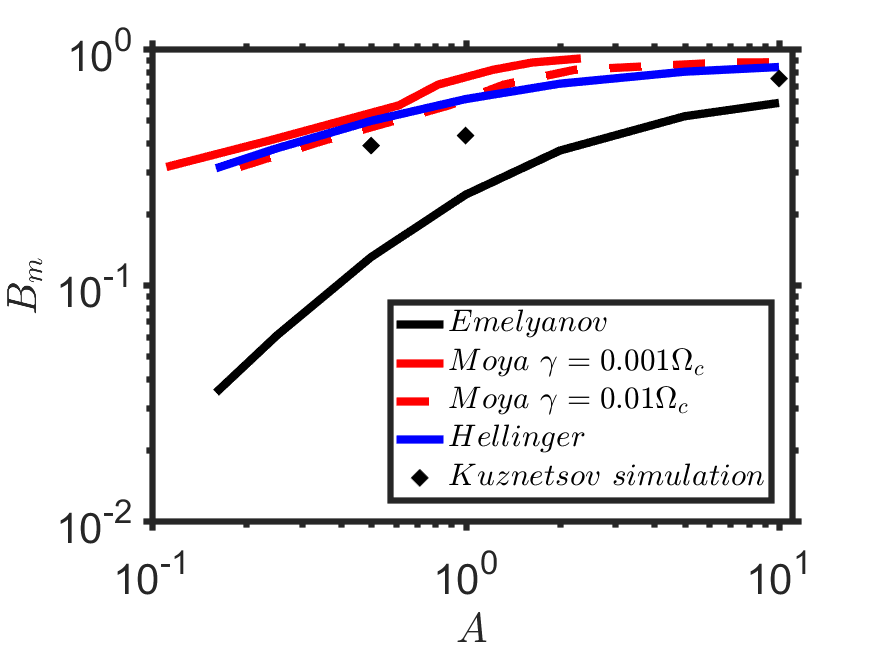
\includegraphics[width=0.5\linewidth]{introduction/b_podavl12.png}
\centering
\captionstyle{normal}
\caption{Зависимость подавляющего внешнего магнитного поля от начальной анизотропии для поперечных апериодических мод~(\ref{eq:Emel_condition}) (черный цвет), всех апериодических мод согласно оценке~(\ref{eq:Hellinger_condition}) (синий цвет) и согласно результатам расчетов~\cite{Moya2022} (красный цвет).}

\label{ris:B_podavl}
\end{figure}

Сравнение оценок (\ref{eq:Emel_condition}) и (\ref{eq:Hellinger_condition}) показывает, что если при высоких начальных анизотропиях отношение $ b_{s}^2/ b_{s\perp}^2$ лишь немного превышает единицу, то при низких начальных анизотропиях оно может составлять несколько порядков~(рис. \ref{ris:B_podavl}). Значит, существует широкий диапазон параметров, в котором принципиально важен учет наклонных мод, так как поперечные моды устойчивы в линейном приближении.

Первая глава работы содержит обсуждение уравнений и посвящена анализу вейбелевской турбулентности в одномерном случае, когда волновой вектор множества учитываемых коллинеарных неустойчивых мод направлен поперек оси анизотропии, т.\,е. вдоль оси $x$. Именно в этом направлении возбуждаются гармоники с наибольшими инкрементами. Для рассматриваемых ТМ-возмущений электрическое поле направлено вдоль оси анизотропии $y$, а магнитное -- вдоль оси $z$.  В данном разделе внимание сосредоточено на механизме возбуждения и насыщения гармоник ФР и магнитного поля, кратных исходной возбуждемой. Продемонстрирована квазилинейность задачи, обеспечивающая возможность пренебрежения высшими кратными гармониками магнитного поля при описании развития вейбелевской турбулентности. Проведено тщательное сравнение полученных численных результатов построенной квазилинейной одномерной модели вейбелевской турбулентности с более ранними аналитическими результатами работы~\cite{Pokhotelov2011}

Во второй главе используются аналогичные квазилинейные уравнения для двумерной задачи и приводятся результаты их решения в простейшем случае аксиальной симметрии, в котором температура частиц и все характеристики вейбелевской турбулентности изотропны в плоскости $xz$, т.е. спектр зависит только от радиальной компоненты $k$ волнового вектора. Эти результаты, полученные для случая двумерной аксиально симметричной турбулентности, сравниваются с полученными методом частиц в ячейках при помощи кода EPOCH~\cite{Arber2015}, учитывающего и более тонкие нелинейные эффекты, в том числе четырехволновое взаимодействие. 

В третье главе при помощи того же квазилинейного приближения описано совместное развитие двухпотоковой (ленгмюровской) и вейбелевской кинетических неустойчивостей в плазме с пучком частиц. Будет показано, что развивающаяся вейбелевская турбулентность магнитного поля может значительно деформировать резонансную с ленгмюровскими волнами область распределения частиц по скоростям, существенно влияя тем самым на формирование и особенно затухание ленгмюровской турбулентности. Ленгмюровская турбулентность электрического поля, в свою очередь, способна существенно изотропизовать распределение частиц по скоростям, а следовательно, изменить инкременты, характер эволюции и уровень насыщения гармоник вейбелевской турбулентности.

В четвертой главе проанализировано  изменение эволюции распределения частиц по скоростям, среднеквадратичного магнитного поля, его спектра в целом и отдельных гармоник в частности с увеличением величины внешнего магнитного поля от малого до почти подавляющего неустойчивость для представительного диапазона величин начальной анизотропии распределения частиц по скоростям. Основное внимание уделяется описанию  процессов нелинейного, в частности, трех- и четырехволнового взаимодействия между модами. В заключительном разделе суммируются общие свойства эволюции квазимагнитостатической турбулентности, генерируемой шланговой неустойчивостью во внешнем магнитном поле, и обсуждается возможная роль этой турбулентности в формировании корональных вспышек на Солнце и звездах поздних спектральных классов.

В пятой главе рассматривается аналогичная постановка задачи для\\ бикаппа-распределения~\cite{Livadiotis2017, Livadiotis2021}, выбранного в качестве начального. Оно свойственно неравновесной плазме, частицы которой испытали стохастическое ускорение под действием того или иного широкополосного электромагнитного излучения, например в звездном ветре или различных ударных волнах, и в качестве частного случая содержит бимаксвелловское распределение частиц по скоростям. Исследования нелинейной стадии вейбелевской неустойчивости для начального бикаппа-распределения ранее отсутствовали.



